\appendix
% Tell TexCount to ignore words in word count
%TC:ignore
\clearpage
\restoregeometry
\newpage
\section{Table of Gestures and Variations}\label{app:gestures}
\textbf{Head Gestures}
\begin{description}
    \item[Pointing-Rotate]\nl
    Turn your head such that the desired content is in the centre of your vision. E.g. if the target is in the bottom right corner of the screen, turn your head down and to the right\\
    \textbfit{Directions:} Up, Up-Right, Right, Down-Right, Down, Down-Left, Left, Up-Left
    \item[Circular]\nl
    Turn your head such that the path of motion of your nose draws a circle.\\
    \textbfit{Directions:} Clockwise, Anti-Clockwise
    \item[Zoom]\nl
    Move your head directly towards or away from the phone screen.\\
    \textbfit{Directions:} Zoom-In, Zoom-Out
    \item[Rotate]\nl
    Turn your head such that you are looking beyond the edge of the screen.\\
    \textbfit{Directions:} Up, Right, Down, Left
    \item[Roll]\nl
    Lean your head to the left or right, bringing it towards your shoulder.\\
    \textbfit{Directions:} Clockwise (Right), Anti-Clockwise (Left)
\end{description}\nl
\textbf{Phone Gestures}
\begin{description}
    \item[POINTING-TRANSLATE]\nl
    Move the phone such that the desired content is in the centre of your vision. E.g. if the target is in the bottom right corner of the screen, move the phone up and to the left.\\
    \textbfit{Directions:} Up, Up-Right, Right, Down-Right, Down, Down-Left, Left, Up-Left
    \item[POINTING-ROTATE]\nl
    Turn the phone such that the desired content is in the centre of your vision. E.g. if the target is in the bottom right corner of the screen, twist the phone such that the bottom right corner is brought towards your face.\\
    \textbfit{Directions:} Up, Up-Right, Right, Down-Right, Down, Down-Left, Left, Up-Left
    \item[Translate]\nl
    Move the phone such that the phone is off to the side of your head.\\
    \textbfit{Directions:} Up, Right, Down, Left
    \item[Circular]\nl
    Move the phone such that its path of motion draws a circle.\\
    \textbfit{Directions:} Clockwise, Anti-Clockwise
    \item[Zoom]\nl
    Move the phone directly towards or away from your head.\\
    \textbfit{Directions:} Zoom-In, Zoom-Out
    \item[Roll]\nl
    Twist the phone such that the phone centre is still the same location, but the corners of the phone are moving clockwise or anti-clockwise.\\
    \textbfit{Directions:} Clockwise, Anti-Clockwise
\end{description}
% \begin{table}[H]
%     \centering
%     \caption{Breakdown of Participants}
%     \label{tab:gesture_breakdown}
%     \begin{tabular}{ c | c | c }
%         Gesture & Description & Directions \\
%         \hline
%         POINTING-TRANSLATE-PHONE & 23 & \\
%         1 & 25 & \\
%         2 & 21 & \\
%         3 & 24 & \\
%         4 & 26 & \\
%         5 & 24 & \\
%         6 & 27 & \\
%         7 & 23 & \\
%         \hline
%     \end{tabular}
% \end{table}

% Data Collection App PUML
% \section{Data Collection App Class Diagram}
% \tempnote{puml sequence diagram showing study steps}

% Full Study Protocol
% \section{Study Protocol Diagram}\label{app:protocol}
% \tempnote{puml sequence diagram showing study steps}
\newpage
\section{Study Data Analysis}\label{app:study_data}
\begin{table}
    \centering
    \caption{Frames with head visible, and total time elapsed per gesture and direction}
    \label{tab:gesture_analysis}
    \begin{tabular}{ c | c | c }
        Gesture And Direction & Percentage of Frames Where Head Is Detected & Time Elapsed (seconds) \\
        \hline
        \textbf{CIRCULAR-HEAD} & \textbfit{97.4\%} & \textbfit{3.208} \\
        ANTI-CLOCKWISE & 97.1\% & 3.156 \\
        CLOCKWISE & 97.7\% & 3.261 \\
        \hline
        \textbf{CIRCULAR-PHONE} & \textbfit{96.1\%} & \textbfit{3.618} \\
        ANTI-CLOCKWISE & 95.9\% & 3.451 \\
        CLOCKWISE & 96.4\% & 3.785 \\
        \hline
        \textbf{POINTING-ROTATE-HEAD} & \textbfit{97.2\%} & \textbfit{2.466} \\
        BOTTOM-CENTRE & 95.3\% & 2.489 \\
        BOTTOM-LEFT & 99.9\% & 2.522 \\
        BOTTOM-RIGHT & 97.4\% & 2.463 \\
        MID-LEFT & 98.9\% & 2.460 \\
        MID-RIGHT & 100\% & 2.392 \\
        TOP-CENTRE & 92.0\% & 2.552 \\
        TOP-LEFT & 96.0\% & 2.319 \\
        TOP-RIGHT & 97.8\% & 2.530 \\
        \hline
        \textbf{POINTING-ROTATE-PHONE} & \textbfit{64.6\%} & \textbfit{2.537} \\
        BOTTOM-CENTRE & 61.9\% & 2.580 \\
        BOTTOM-LEFT & 61.7\% & 2.511 \\
        BOTTOM-RIGHT & 68.6\% & 2.362 \\
        MID-LEFT & 56.1\% & 2.480 \\
        MID-RIGHT & 57.4\% & 2.604 \\
        TOP-CENTRE & 90.2\% & 2.641 \\
        TOP-LEFT & 60.3\% & 2.563 \\
        TOP-RIGHT & 60.3\% & 2.554 \\
        \hline
        \textbf{POINTING-TRANSLATE-PHONE} & \textbfit{95.6\%} & \textbfit{2.865} \\
        BOTTOM-CENTRE & 98.6\% & 2.987 \\
        BOTTOM-LEFT & 96.2\% & 2.639 \\
        BOTTOM-RIGHT & 94.2\% & 2.705 \\
        MID-LEFT & 89.0\% & 2.505 \\
        MID-RIGHT & 94.1\% & 2.621 \\
        TOP-CENTRE & 99.7\% & 3.568 \\
        TOP-LEFT & 95.0\% & 2.828 \\
        TOP-RIGHT & 98.1\% & 3.051 \\
        \hline
        \textbf{ROTATE-HEAD} & \textbfit{85.9\%} & \textbfit{2.843} \\
        BOTTOM-CENTRE & 84.6\% & 2.841 \\
        MID-LEFT & 94.1\% & 2.723 \\
        MID-RIGHT & 92.7\% & 2.837 \\
        TOP-CENTRE & 71.6\% & 2.975 \\
        \hline
        \textbf{ROTATE-HEAD-ROLL} & \textbfit{96.7\%} & \textbfit{2.996} \\
        ANTI-CLOCKWISE & 96.2\% & 2.985 \\
        CLOCKWISE & 97.2\% & 3.007 \\
        \hline
        \textbf{ROTATE-PHONE-ROLL} & \textbfit{87.8\%} & \textbfit{2.799} \\
        ANTI-CLOCKWISE & 78.7\% & 2.763 \\
        CLOCKWISE & 96.9\% & 2.835 \\
        \hline
        \textbf{TRANSLATE-PHONE} & \textbfit{80.9\%} & \textbfit{2.898} \\
        BOTTOM-CENTRE & 85.0\% & 2.902 \\
        MID-LEFT & 71.3\% & 2.918 \\
        MID-RIGHT & 70.3\% & 2.847 \\
        TOP-CENTRE & 96.4\% & 2.925 \\
        \hline
        \textbf{ZOOM-HEAD} & \textbfit{88.1\%} & \textbfit{3.072} \\
        ZOOM-IN & 79.9\% & 3.146 \\
        ZOOM-OUT & 96.3\% & 2.998 \\
        \hline
        \textbf{ZOOM-PHONE} & \textbfit{89.6\%} & \textbfit{3.246} \\
        ZOOM-IN & 82.6\% & 3.247 \\
        ZOOM-OUT & 96.6\% & 3.245 \\
        \hline
    \end{tabular}
\end{table}

% \begin{figure}
%     \centering
%     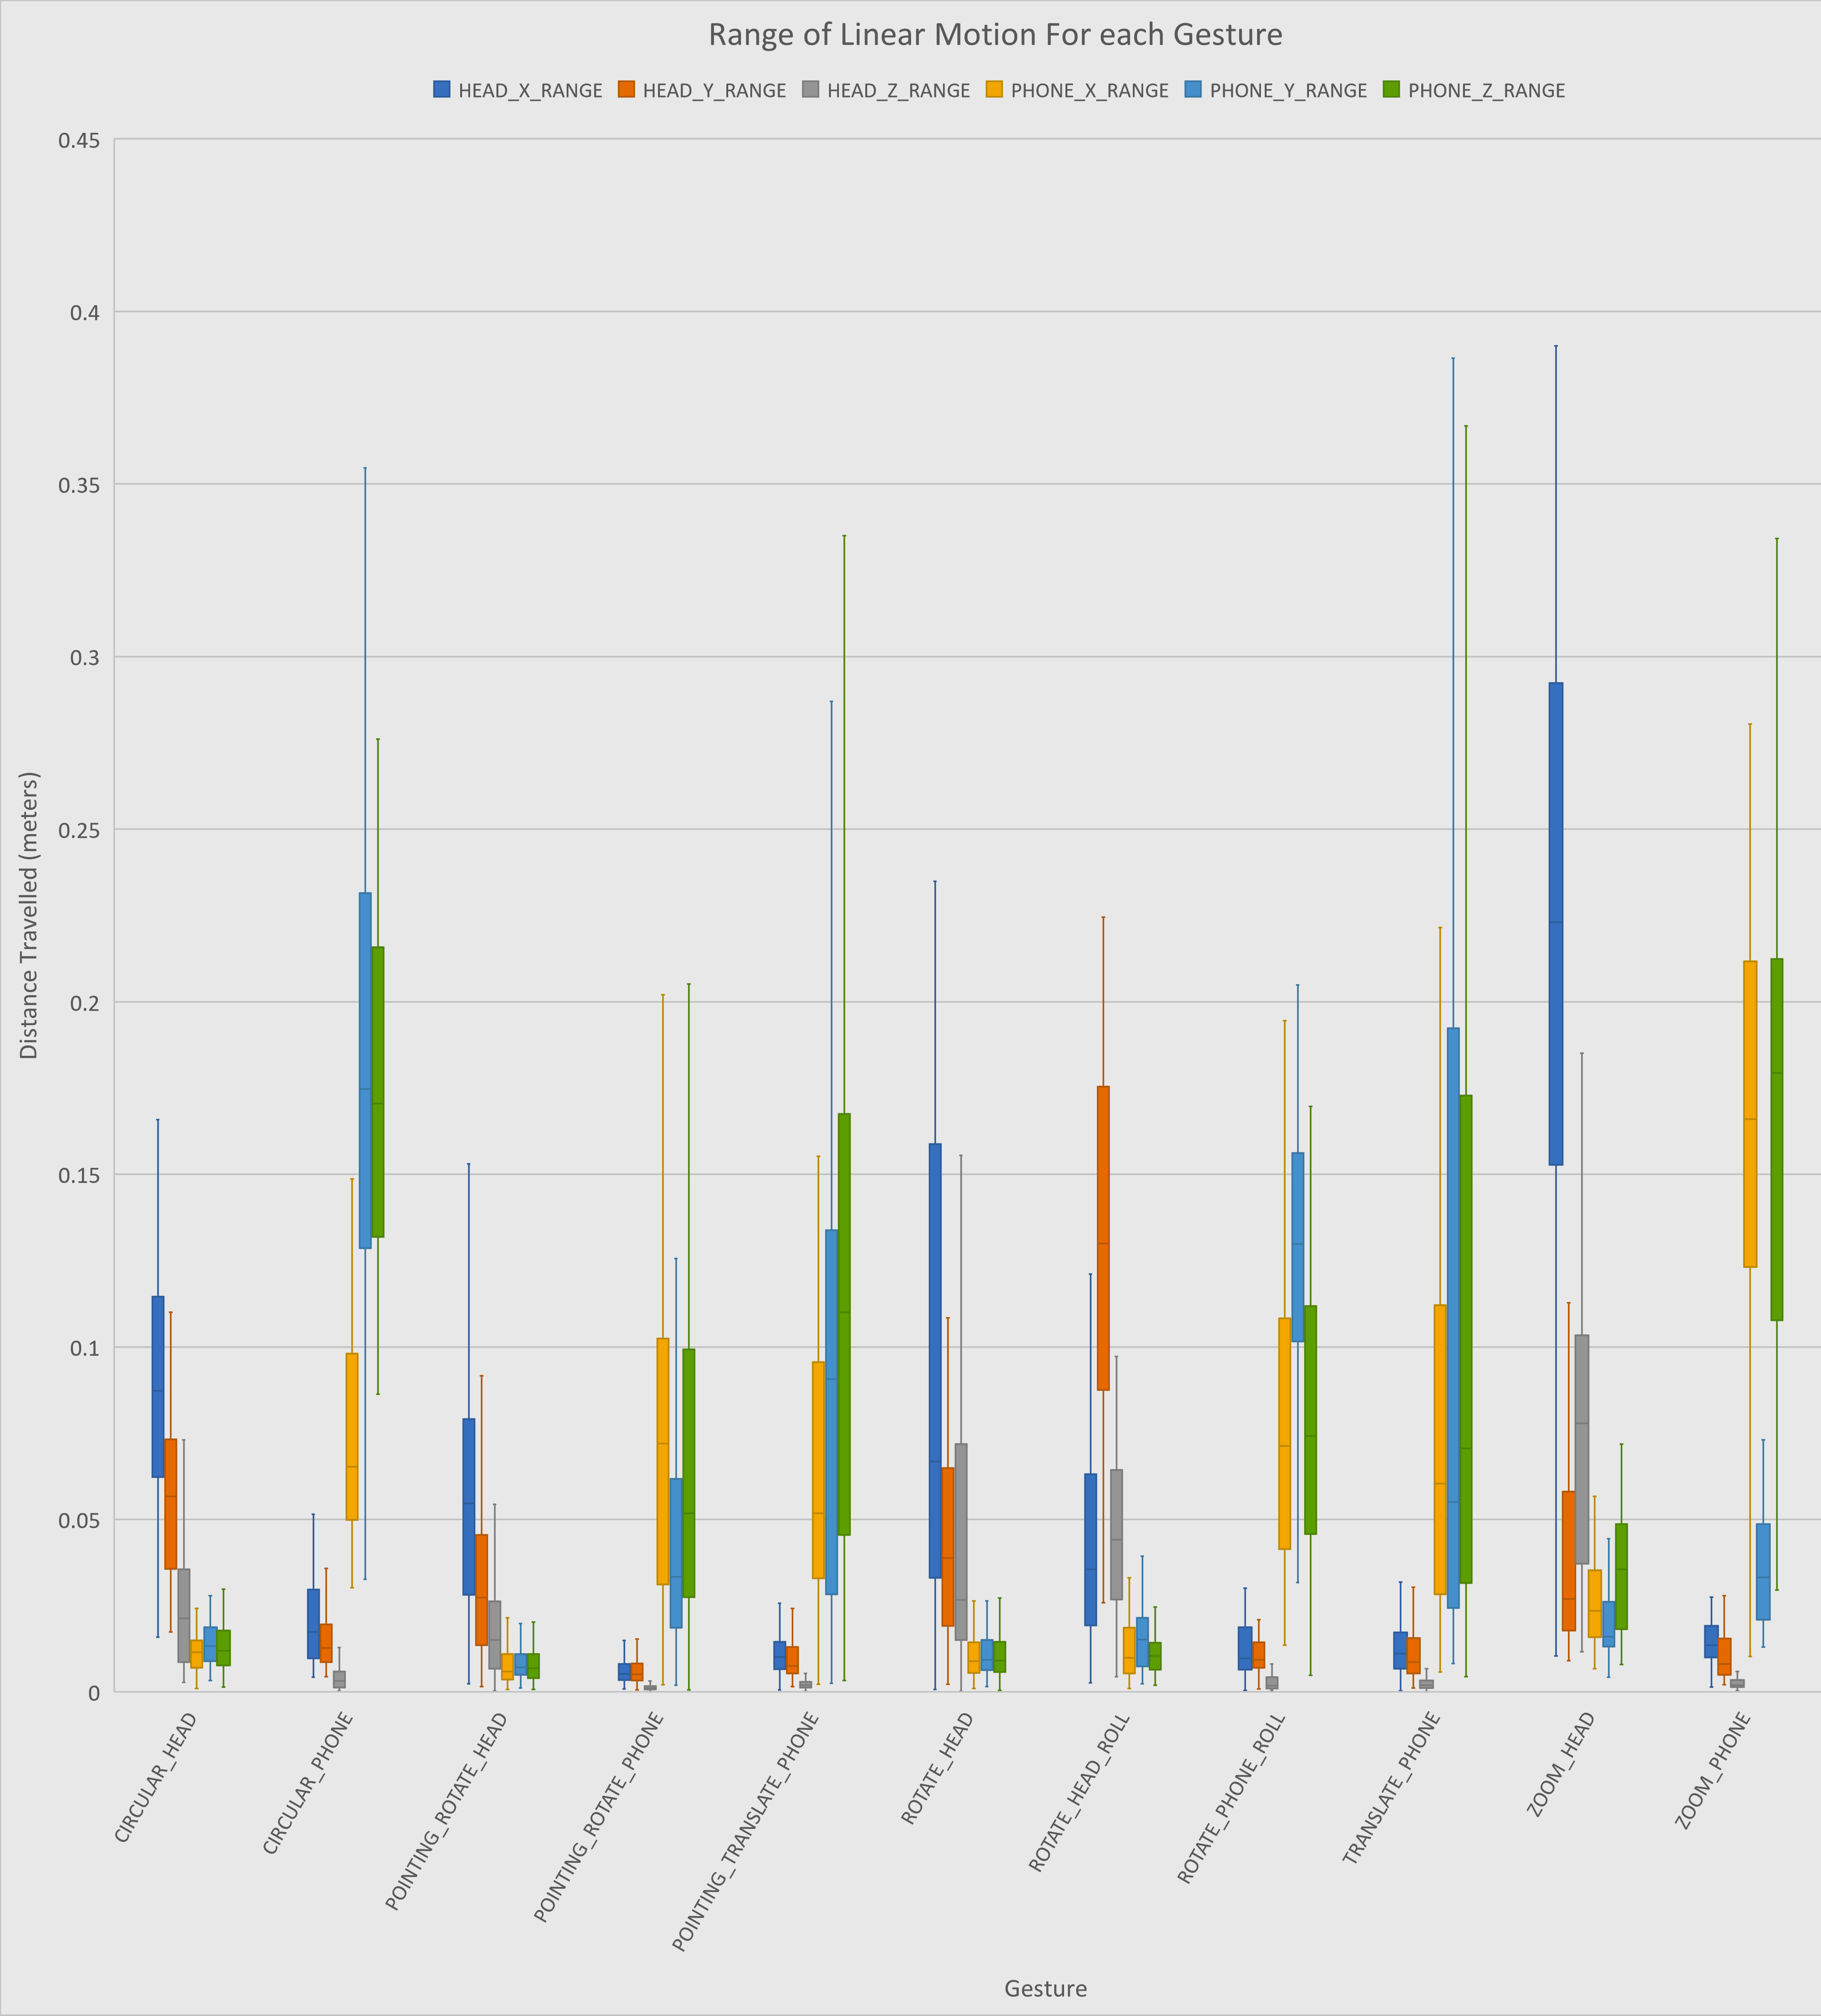
\includegraphics[width=\textwidth]{figures/RangeOfLinearMotion.png}
%     \caption{\label{fig:range_of_linear_motion} Range of linear motion for each gesture, in meters}
%     \Description{Box and Wisker plot showing the mean, min, max, and the first and third quartiles for the observed range of linear motion for each gesture recorded.}
% \end{figure}

\begin{figure}[H]
    \centering
    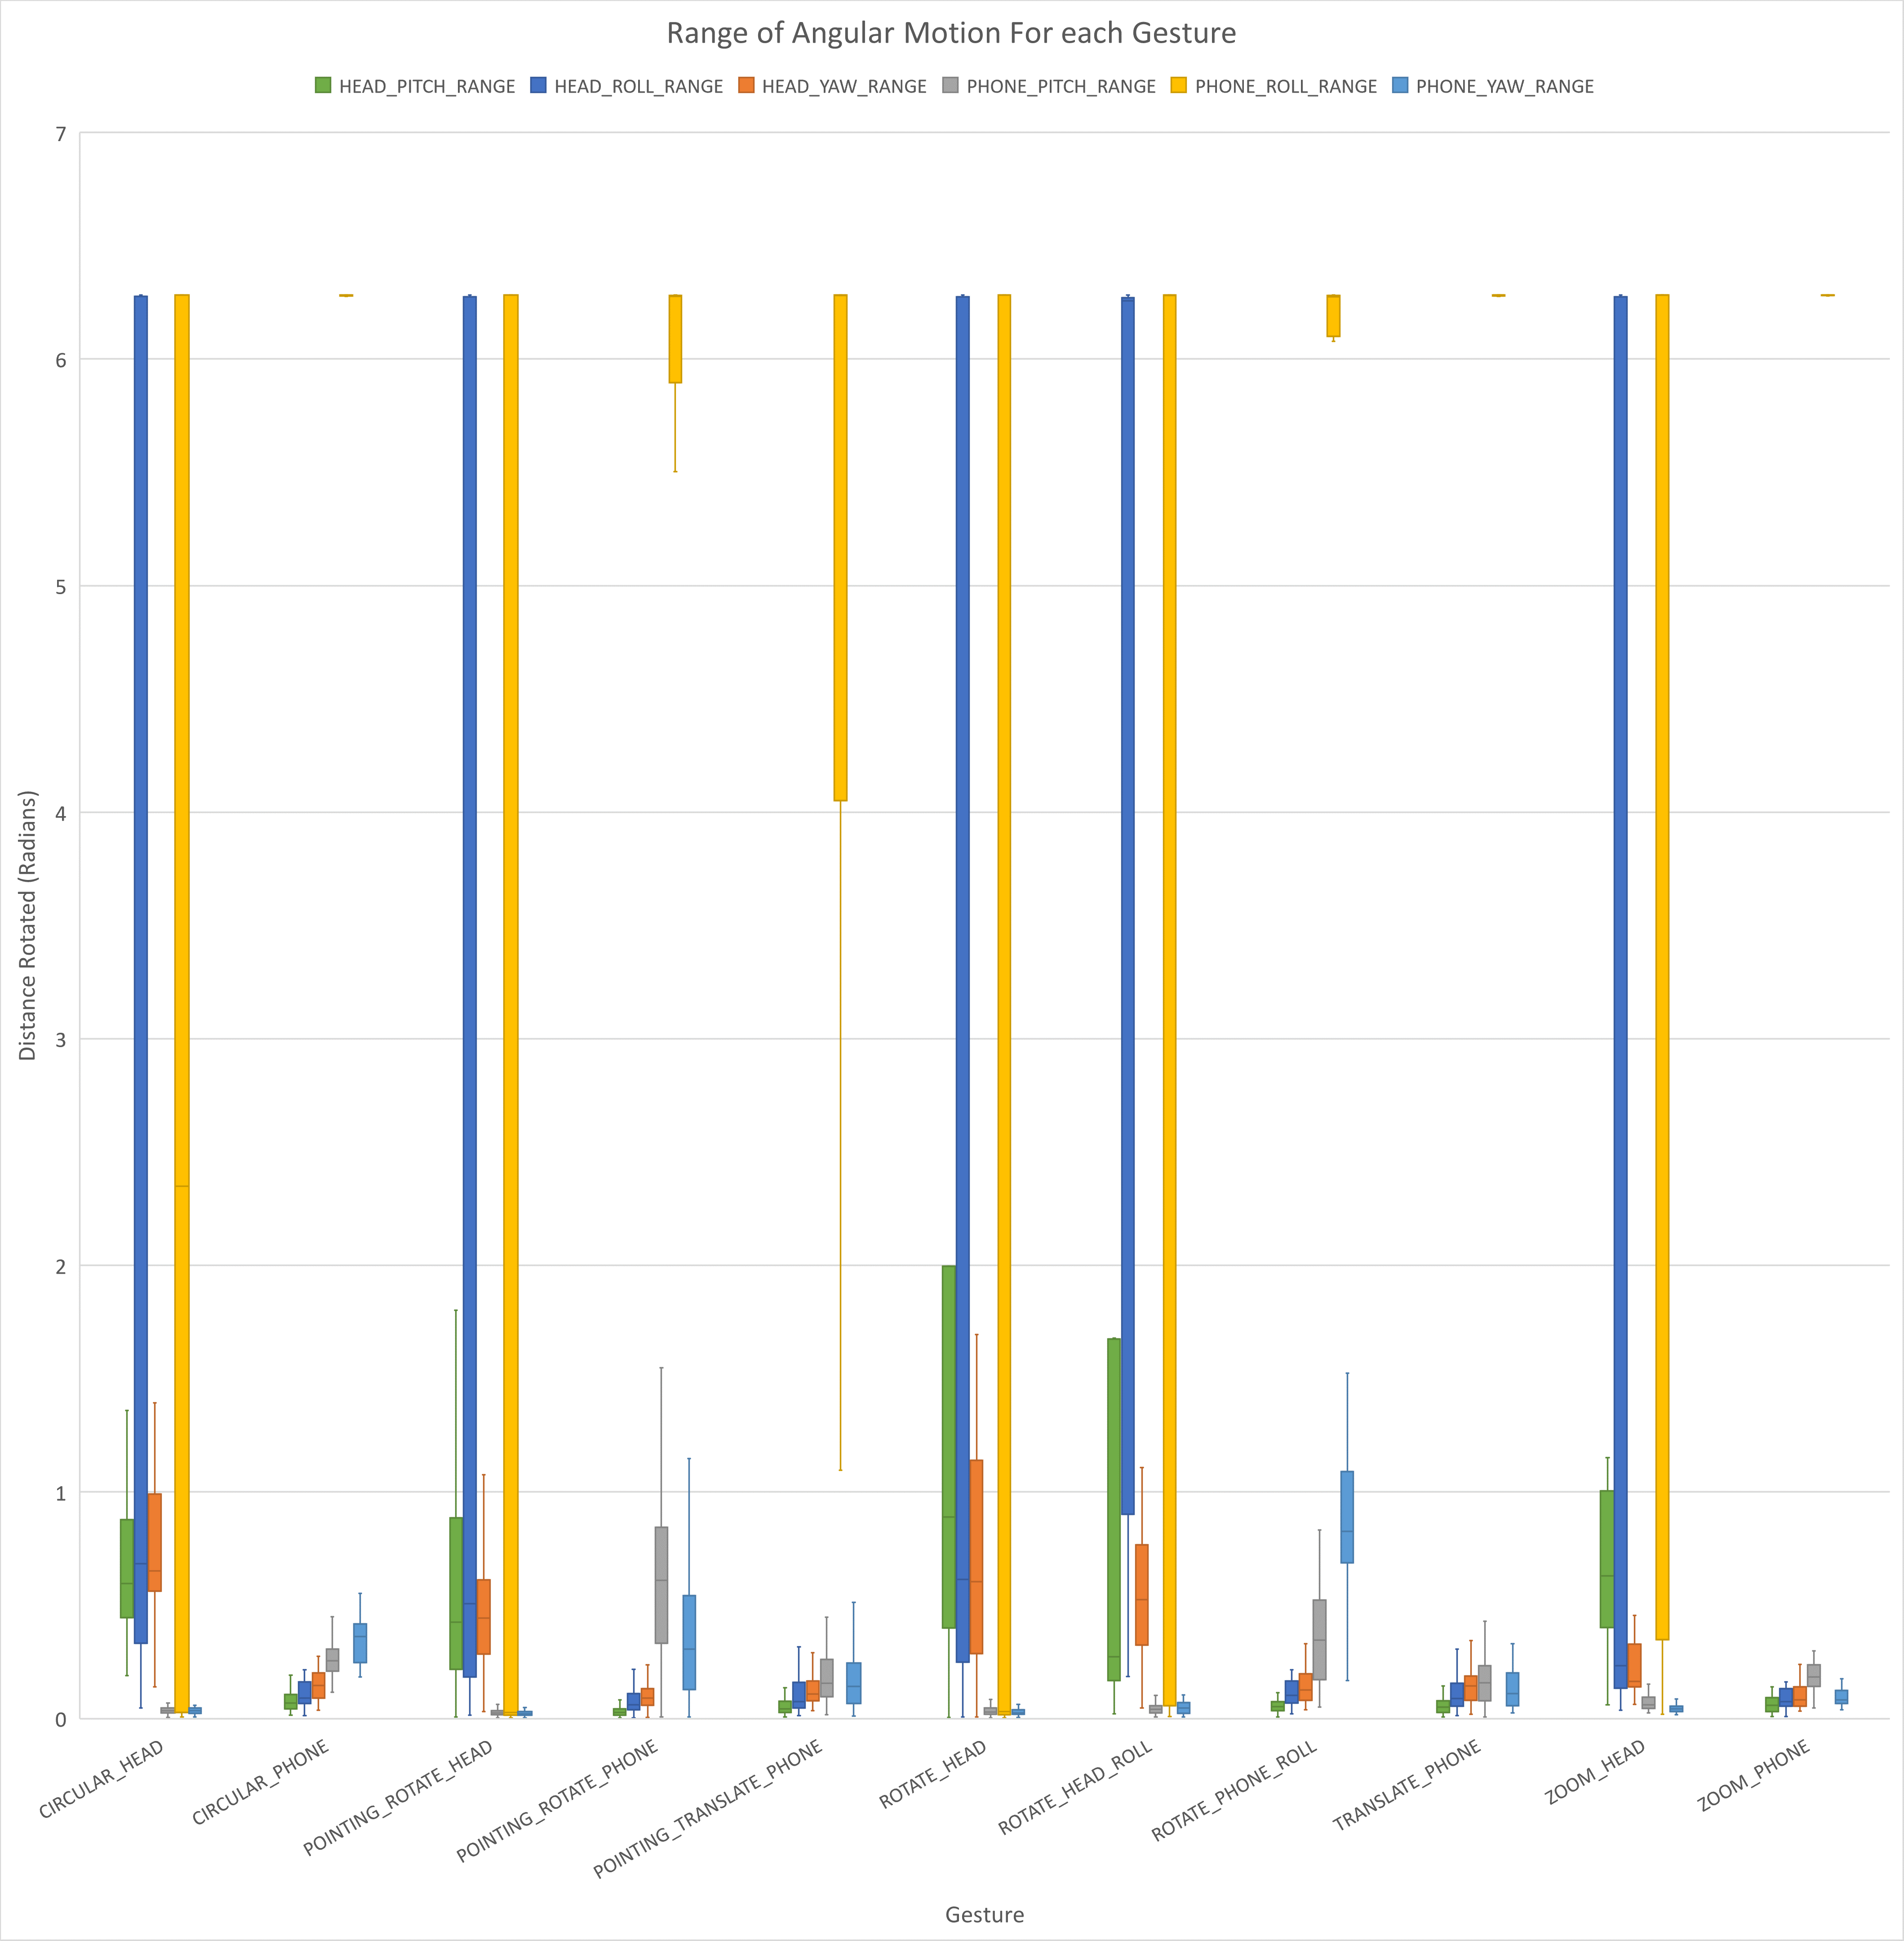
\includegraphics[width=\textwidth]{figures/RangeOfAngularMotion.png}
    \caption{\label{fig:range_of_angular_motion} Range of angular motion for each gesture, in meters}
    \Description{Box and Wisker plot showing the mean, min, max, and the first and third quartiles for the observed range of angular motion for each gesture recorded.}
\end{figure}

% Tell TexCount to start counting words again
%TC:endignore
